\documentclass{beamer}

\usepackage{BeamerThemePittsburgh}

\usepackage{graphicx}
\usepackage{listings}

\usepackage{hyperref}
\hypersetup{
    colorlinks=true,
    linkcolor=blue,
    filecolor=magenta,      
    urlcolor=cyan,
    }

\begin{document}

\title{MPSGE.jl}
\author{Mitch Phillipson \inst{1} \and Eli Lazarus \inst{2}}
\institute[shortinst]{\inst{1} University of Wisconsin-Madison \and \inst{2} Stanford University}


\date{April 22, 2025}

\maketitle


\begin{frame}{Closed $2\times 2$ Economy}

    This is adapted from \href{https://mpsge.org/tutorial.pdf}{Jim Markusen's} example `M22`. This model introduces intermediate goods and a simple CES nesting that permits specification of different elasticities of substitution between different groups of inputs. 

    \pause
    \vspace{1cm}

    \begin{center}
        \begin{tabular}{ccccc}
                  & X     & Y     & W      & CONS    \\ \hline
            $PX$  & $120$ & $-20$ & $-100$ & $0   $  \\
            $PY$  & $-20$ & $120$ & $-100$ & $0   $  \\
            $PW$  & $0  $ & $0  $ & $200 $ & $-200$  \\
            $PK$  & $-60$ & $-40$ & $0   $ & $100 $  \\
            $PL$  & $-40$ & $-60$ & $0   $ & $100 $  
        \end{tabular}
    \end{center}

\end{frame}


\begin{frame}{Closed $2\times 2$ Economy}

    \begin{minipage}{.2\textwidth}
        \begin{tabular}{cc}
            & X             \\ \hline
            $PX$  & $120$   \\
            $PY$  & $-20$   \\
            $PW$  & $0  $   \\
            $PK$  & $-60$   \\
            $PL$  & $-40$   
        \end{tabular}
    \end{minipage}
    \hfill \pause
    \begin{minipage}{.78\textwidth}
        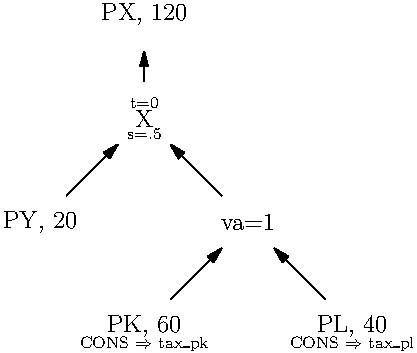
\includegraphics[width=\textwidth]{images/x_sector.pdf}
    \end{minipage}
\end{frame}


\begin{frame}[fragile]{Closed $2\times 2$ Economy}

    Let's set up an environment and install the packages we need. Start Julia from the directory where you want to work. 

    \begin{verbatim}
julia> ]
pkg> activate .
pkg> add MPSGE, JuMP, PATHSolver, PlotlyJS, DataFrames
pkg> dev https://github.com/julia-mpsge/markusen_2_2.jl
    \end{verbatim}

    We've added the \texttt{markusen\_2\_2} as \emph{dev}, typically you want to do this with packages in your personal GitHub as \emph{dev} stands for \emph{development}. Best practice would be to fork the repo and dev the fork, but we will survive without that for now.

    \vspace{.5cm}

    Alternatively, you can just \emph{add} the \texttt{markusen\_2\_2} package, it's just a little easier to view the source code if you have it in your local environment.

\end{frame}

\begin{frame}{Closed $2\times 2$ Economy}
    Before going further, ensure that VSCode is using the environment we just defined. On the bottom of VSCode is a blue bar, on the left should be the text \texttt{Julia env: } with the active environment. If it isn't your working directory click on it and select the environment you just created.

    \vspace{.5cm}

    The README in the GitHub repo has an \href{https://github.com/julia-mpsge/markusen\_2\_2.jl\#example-code}{example} using the code, just copy/paste that into a file and save it as \texttt{markusen.jl}.
\end{frame}


\begin{frame}[fragile]{Closed $2\times 2$ Economy}

    Let's look at the models. You can either do this directly on GitHub, which is the easiest method, or you can open the directory.

    \vspace{.5cm}

    If you used dev, then the source code is located in:

    \begin{verbatim}
    ~/.julia/dev/markusen_2_2
    \end{verbatim}

    \vspace{.5cm}

\end{frame}


\begin{frame}{Closed $2\times 2$ Economy}
    \begin{minipage}{.95\textwidth}
        \centering
        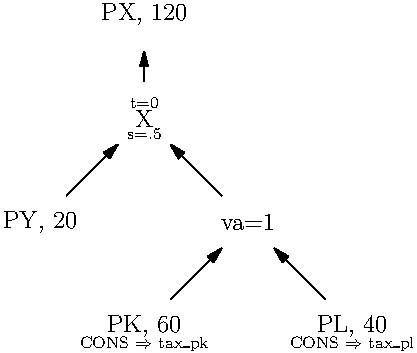
\includegraphics[width=\textwidth]{images/x_sector.pdf}
    \end{minipage}
\end{frame}


\begin{frame}[fragile]{WiNDC Household Model}

    First, add the package to your environment. \href{https://github.com/julia-mpsge/windc_household_model.jl}{Here is a link to the GitHub repo.}

    \begin{verbatim}
pkg> add https://github.com/julia-mpsge/windc_household_model.jl
    \end{verbatim}


    The household model disaggregates the WiNDC state model into 5 consumers per state, corresponding to the 5 quintiles of income. 

\end{frame}



\end{document}